\section{Eksperimenti 2. faze}
"Opis testa Nowatzky "

Merjenci  so opravili obremenilni test po protokolu Nowatzky. To je stopnjevani test na tekoči preprogi za merjenje maksimalne porabe kisika in oceno aerobne kapacitete  posameznika. Test smo izvajali s pomočjo sistema za direktno ergospirometrijo tipa "breath  by breath" Cosmed K4B2. Uporabili smo  tekočo  preprogo HP Cosmos. Test smo pričeli z ogrevanjem 3 minute s hitrostjo teka 5 km/h, pri naklon preproge 0 \%. Nadaljevali smo s 3 minutnim tekom s hitrostjo 6 km/h. Po treh minutah smo naklon tekoče preproge  dvignili za 2 \% in ga nismo več spreminjali. Po pretečeni minuti na  tretji stopnji (hitrost 6; naklon 2 \%) se je hitrost teka vsaki dve  minuti  povečevala za 1 km/h. Test smo izvajali brez prekinitve do pojava objektivnih oz. subjektivnih razlogov za prekinitev testa. Po koncu testiranja je sledilo še 5 min hoje pri  hitrosti 2 km/h ter 0 \% naklonu.  


\begin{figure}[htb]
\centering
\begin{subfigure}[t]{0.45\columnwidth}
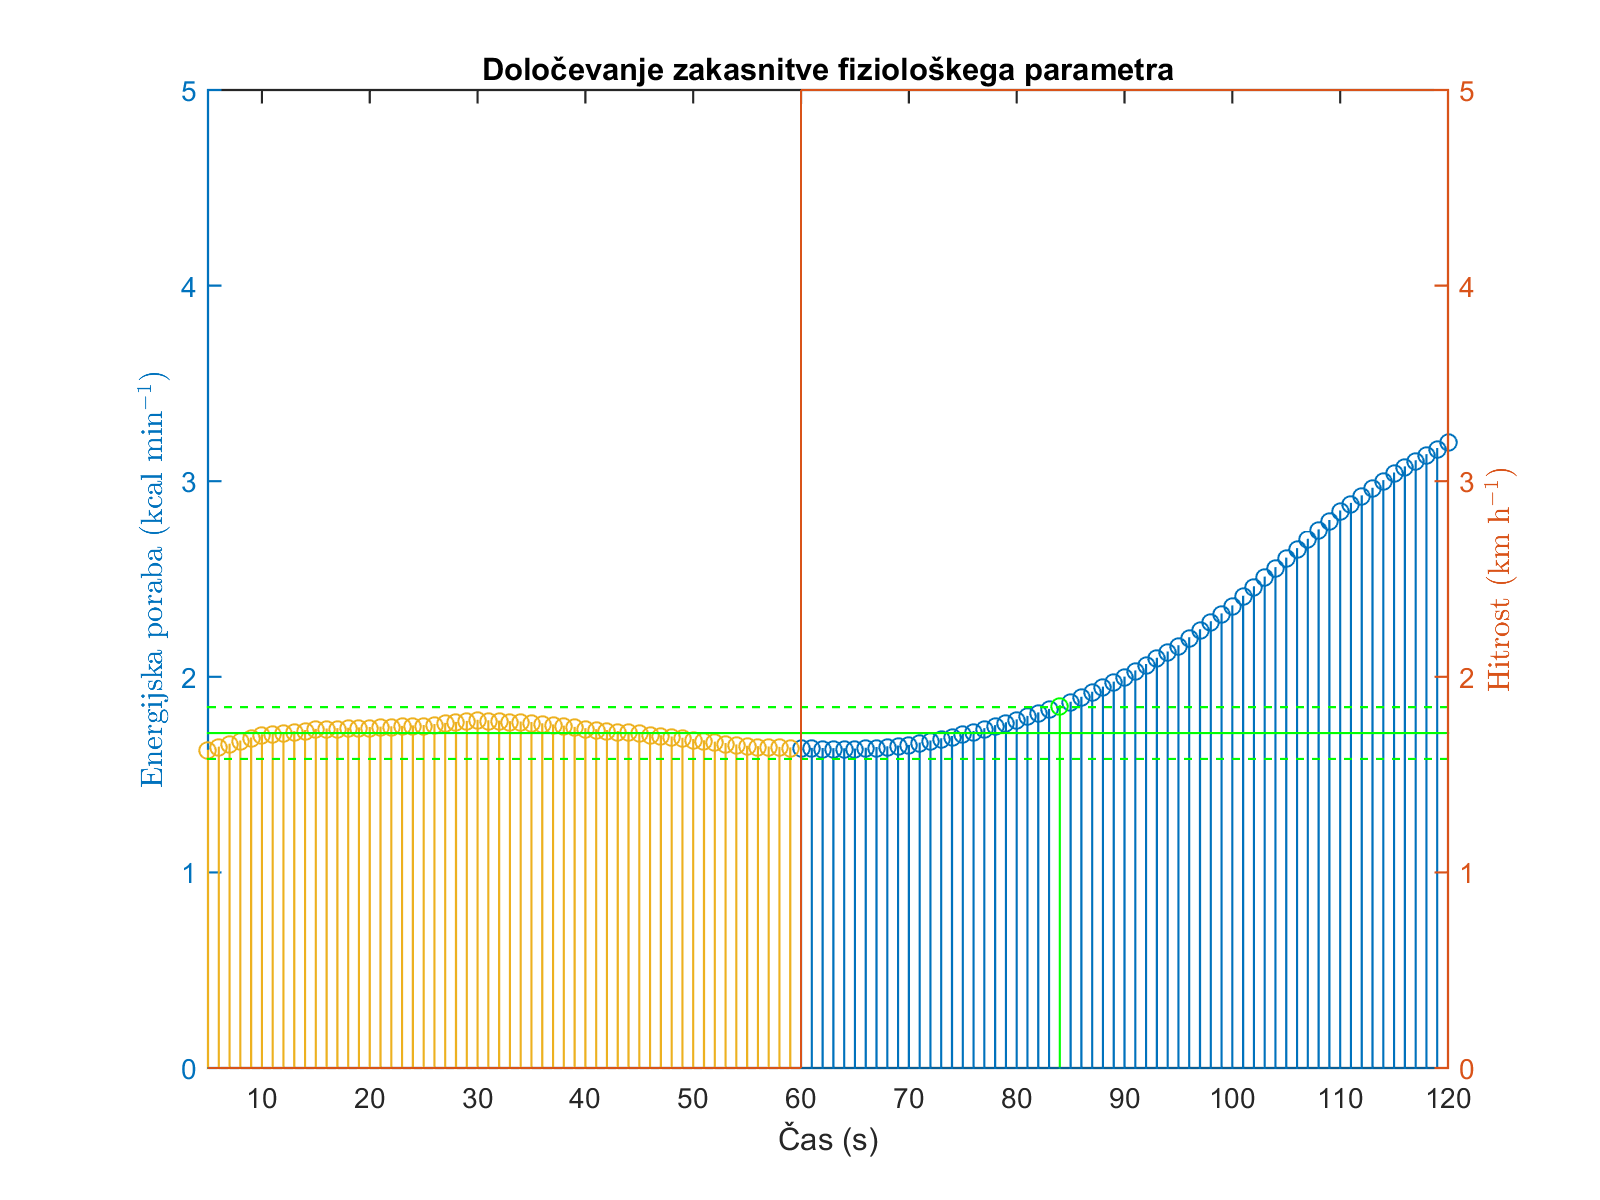
\includegraphics[width=\columnwidth]{./Slike/lag-estimation-1-eem.png}
\caption{Zakasnitev za subjekt 1.}
\label{fig:lag-estimation-train-eem}
\end{subfigure}
~
\begin{subfigure}[t]{0.45\columnwidth}
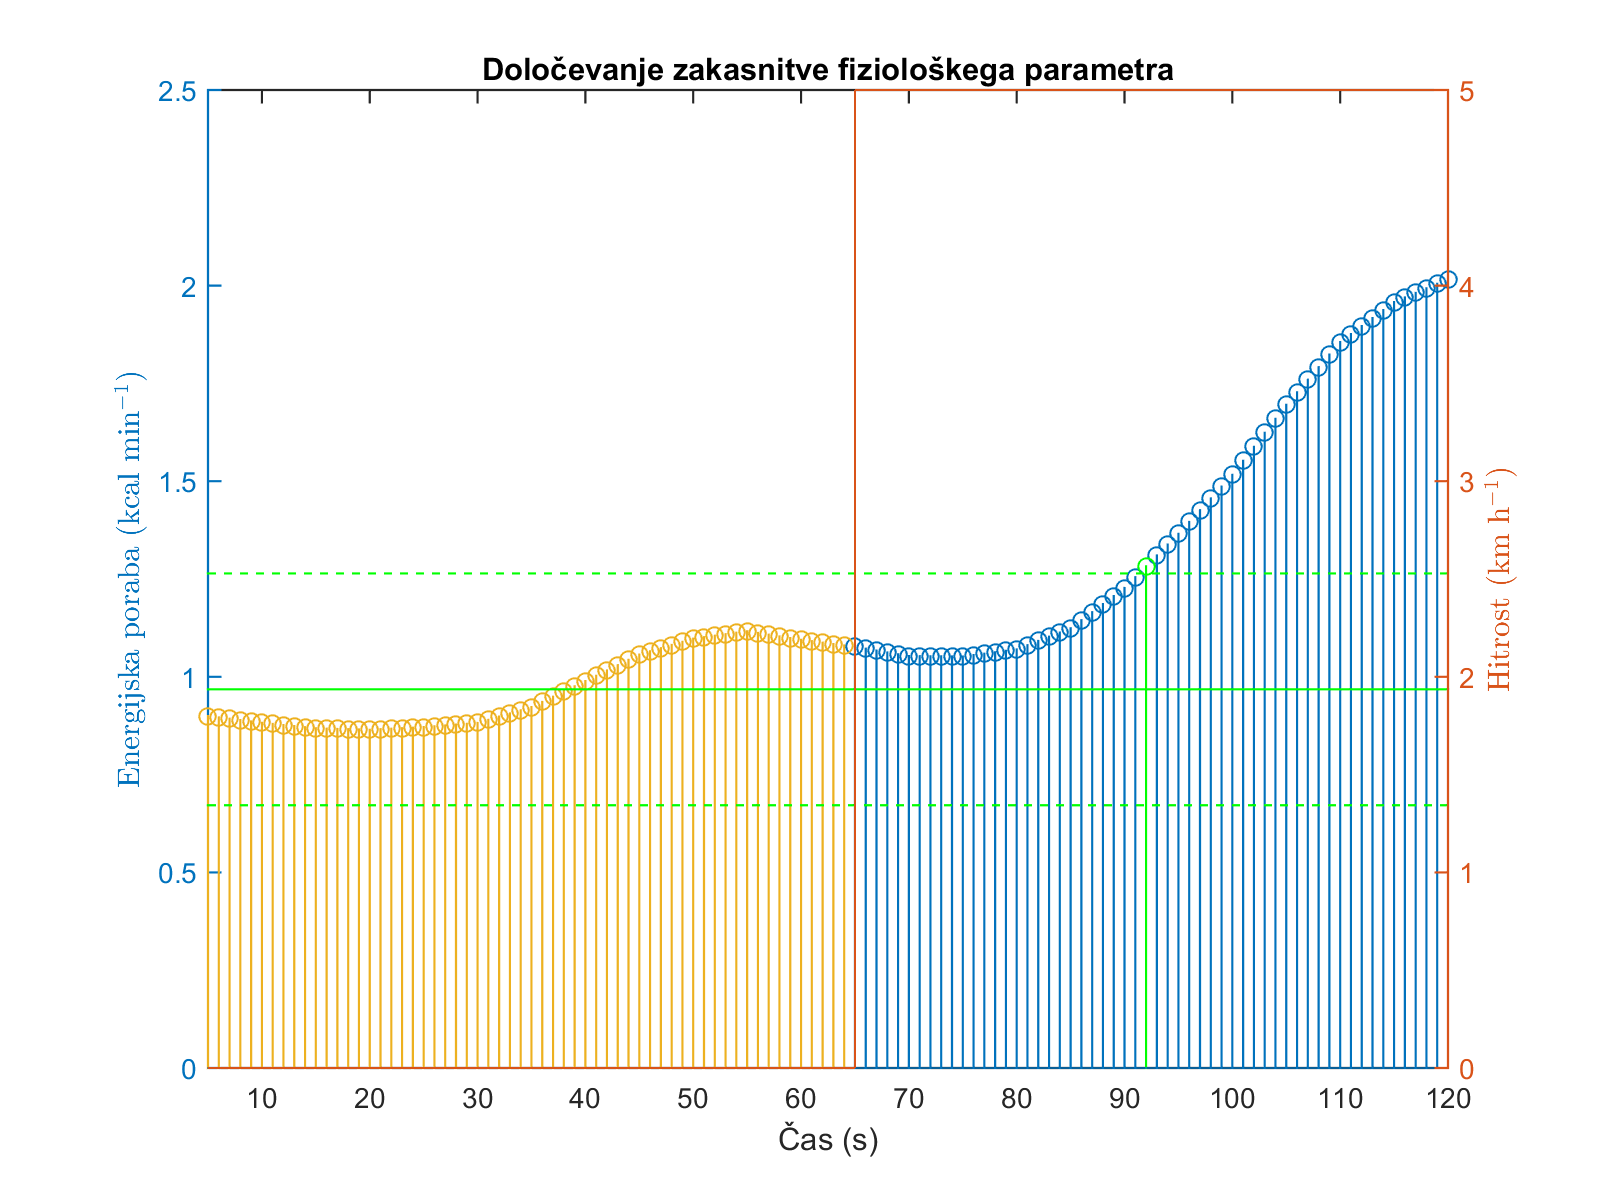
\includegraphics[width=\columnwidth]{./Slike/lag-estimation-2-eem.png}
\caption{Zakasnitev za subjekt 2.}
\label{fig:lag-estimation-train-hr}
\end{subfigure}
~
\begin{subfigure}[t]{0.45\columnwidth}
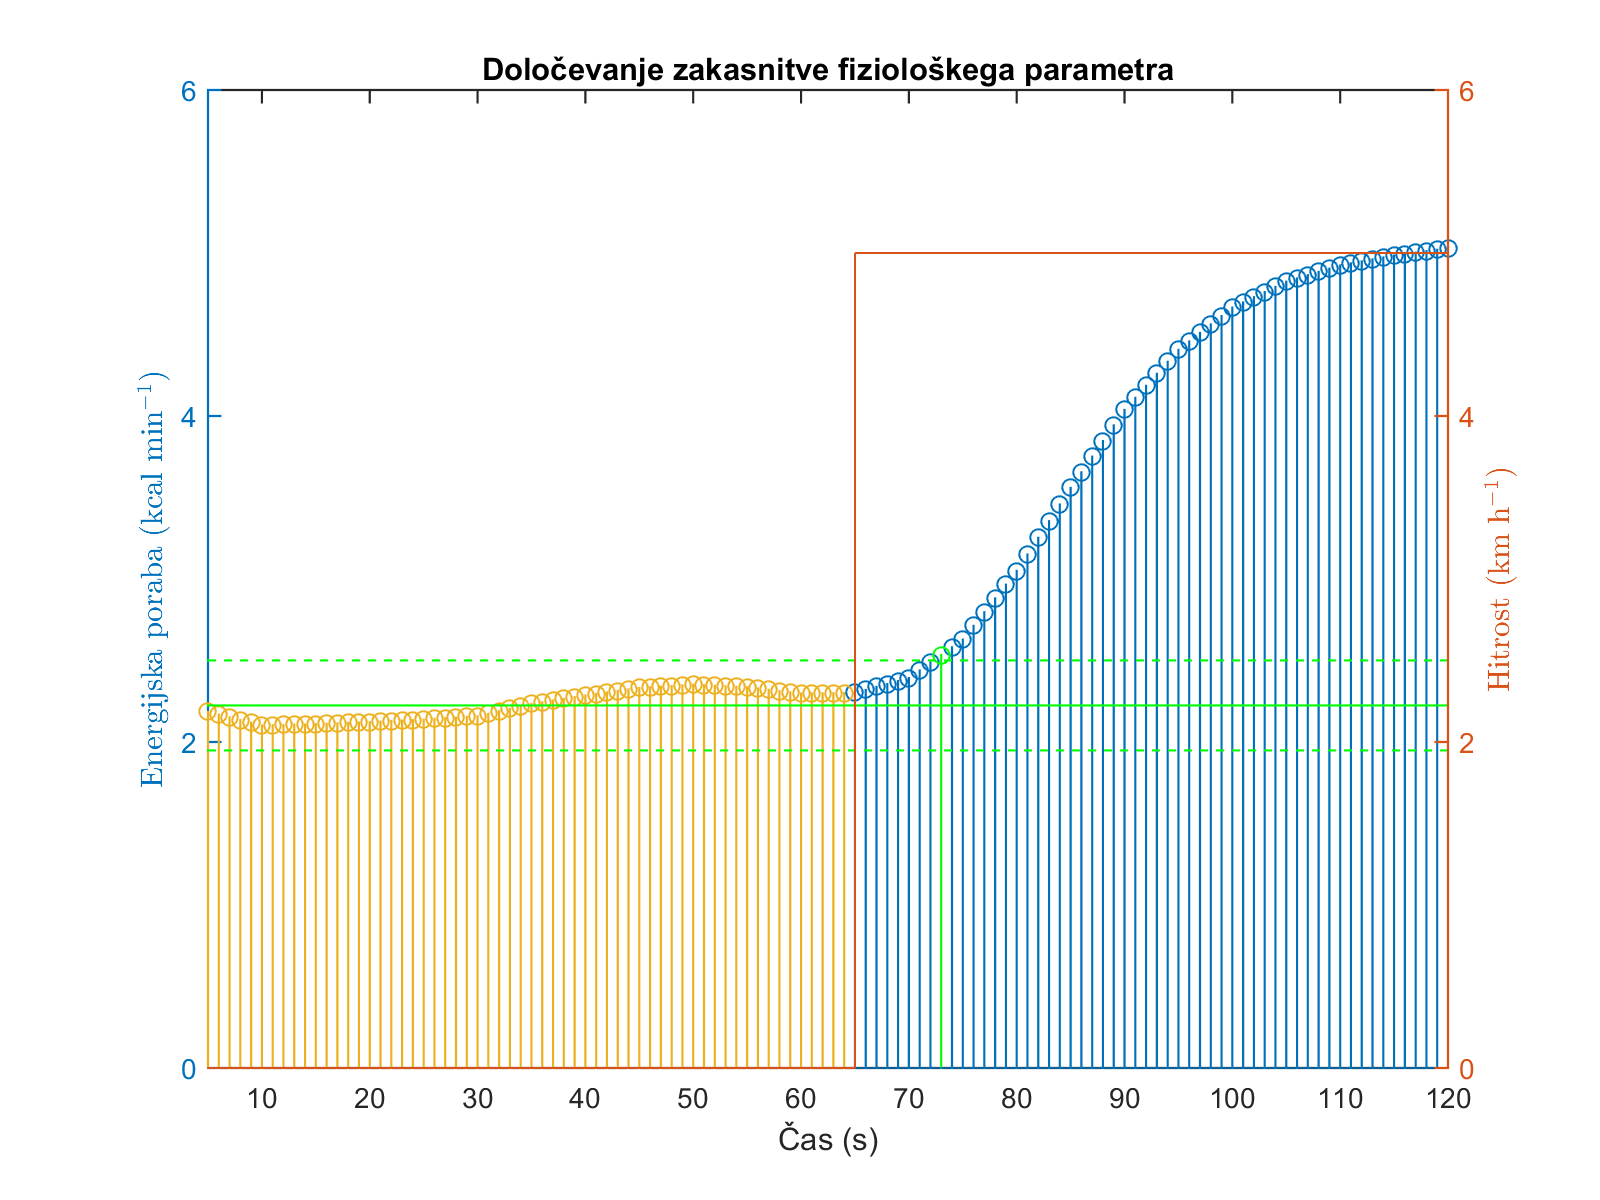
\includegraphics[width=\columnwidth]{./Slike/lag-estimation-3-eem.png}
\caption{Zakasnitev za subjekt 3.}
\label{fig:lag-estimation-train-eem}
\end{subfigure}
~
\begin{subfigure}[t]{0.45\columnwidth}
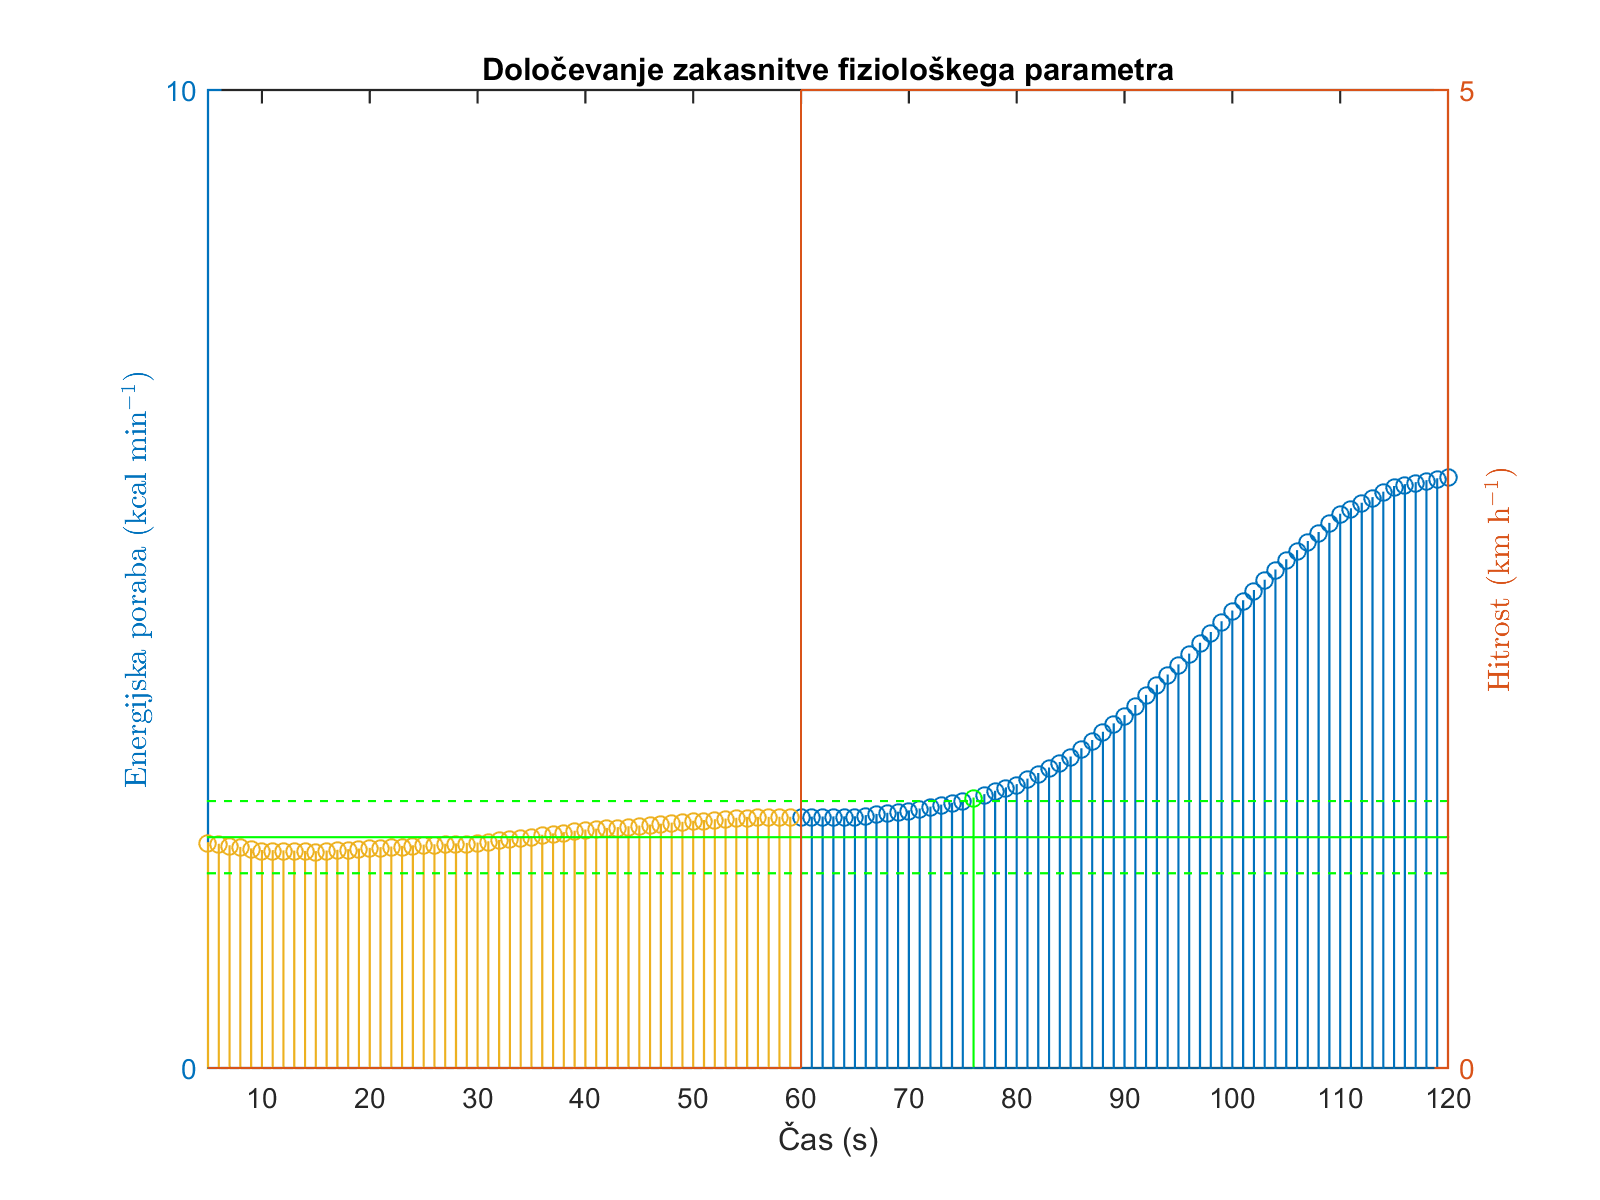
\includegraphics[width=\columnwidth]{./Slike/lag-estimation-4-eem.png}
\caption{Zakasnitev za subjekt 4.}
\label{fig:lag-estimation-train-eem}
\end{subfigure}
~
\begin{subfigure}[t]{0.45\columnwidth}
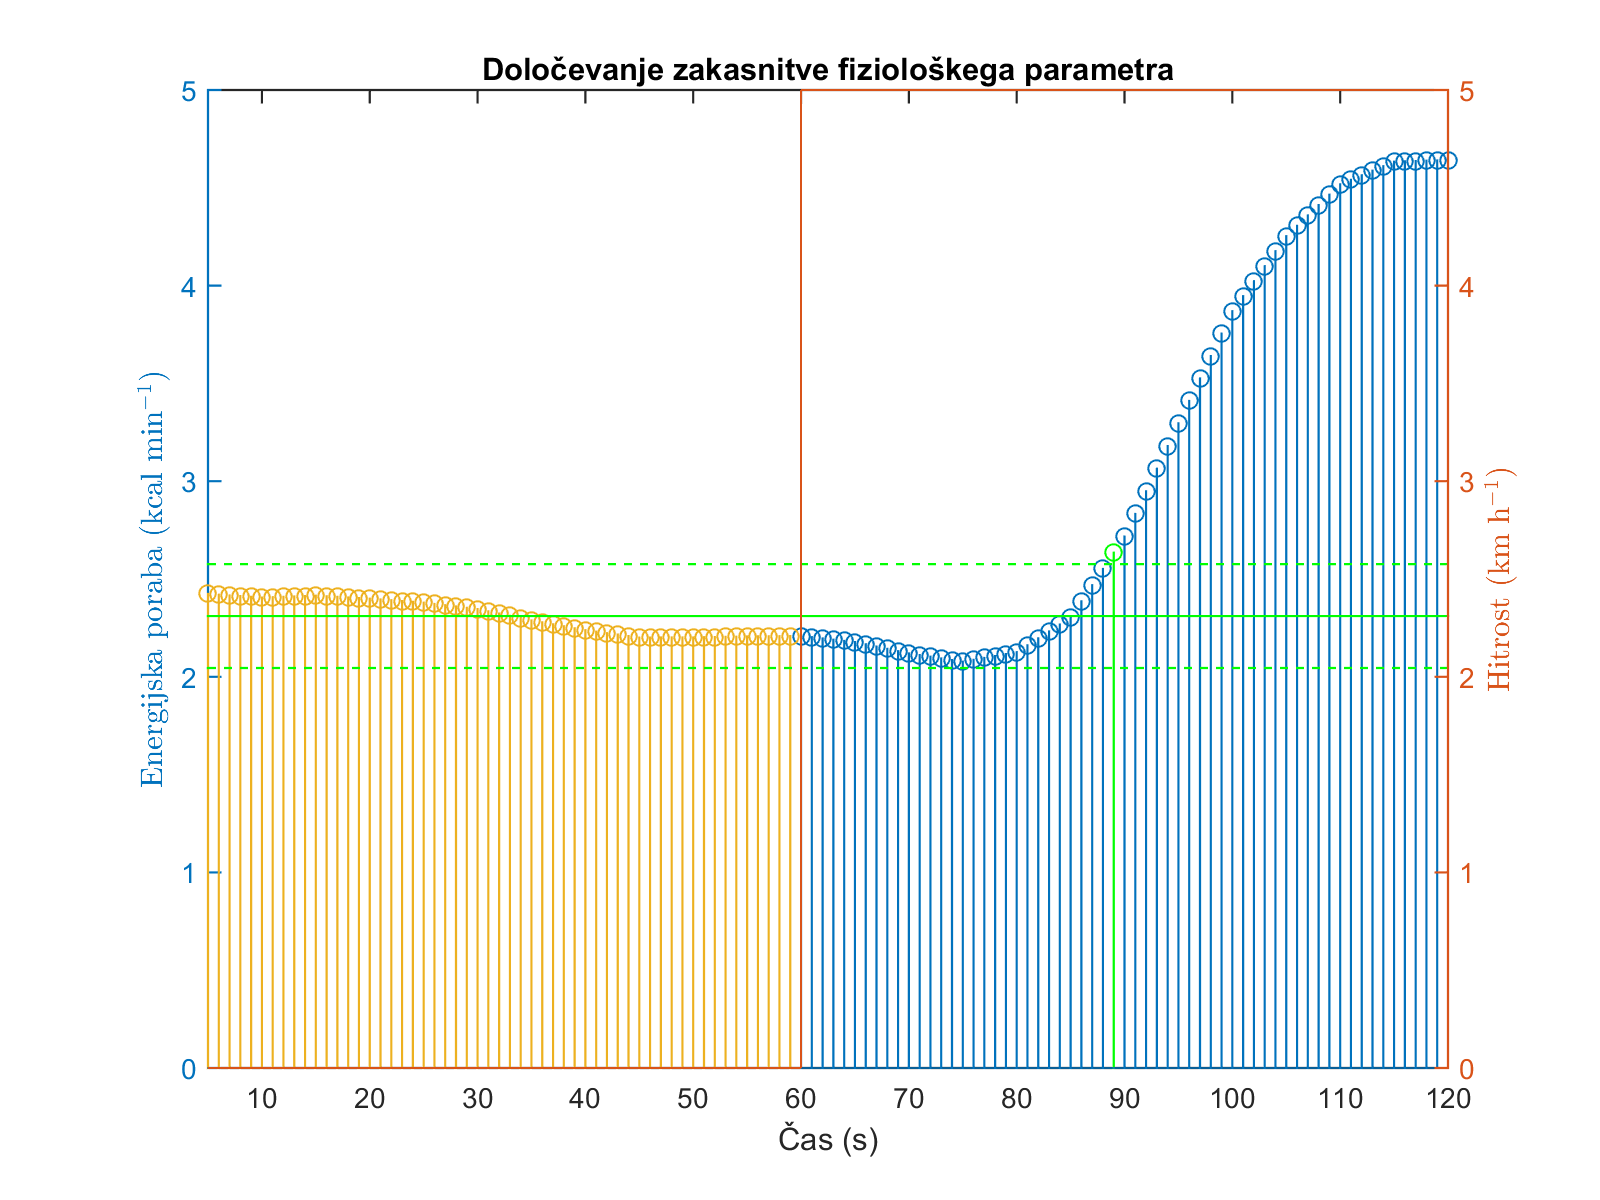
\includegraphics[width=\columnwidth]{./Slike/lag-estimation-5-eem.png}
\caption{Zakasnitev za subjekt 5.}
\label{fig:lag-estimation-train-eem}
\end{subfigure}
~
\begin{subfigure}[t]{0.45\columnwidth}
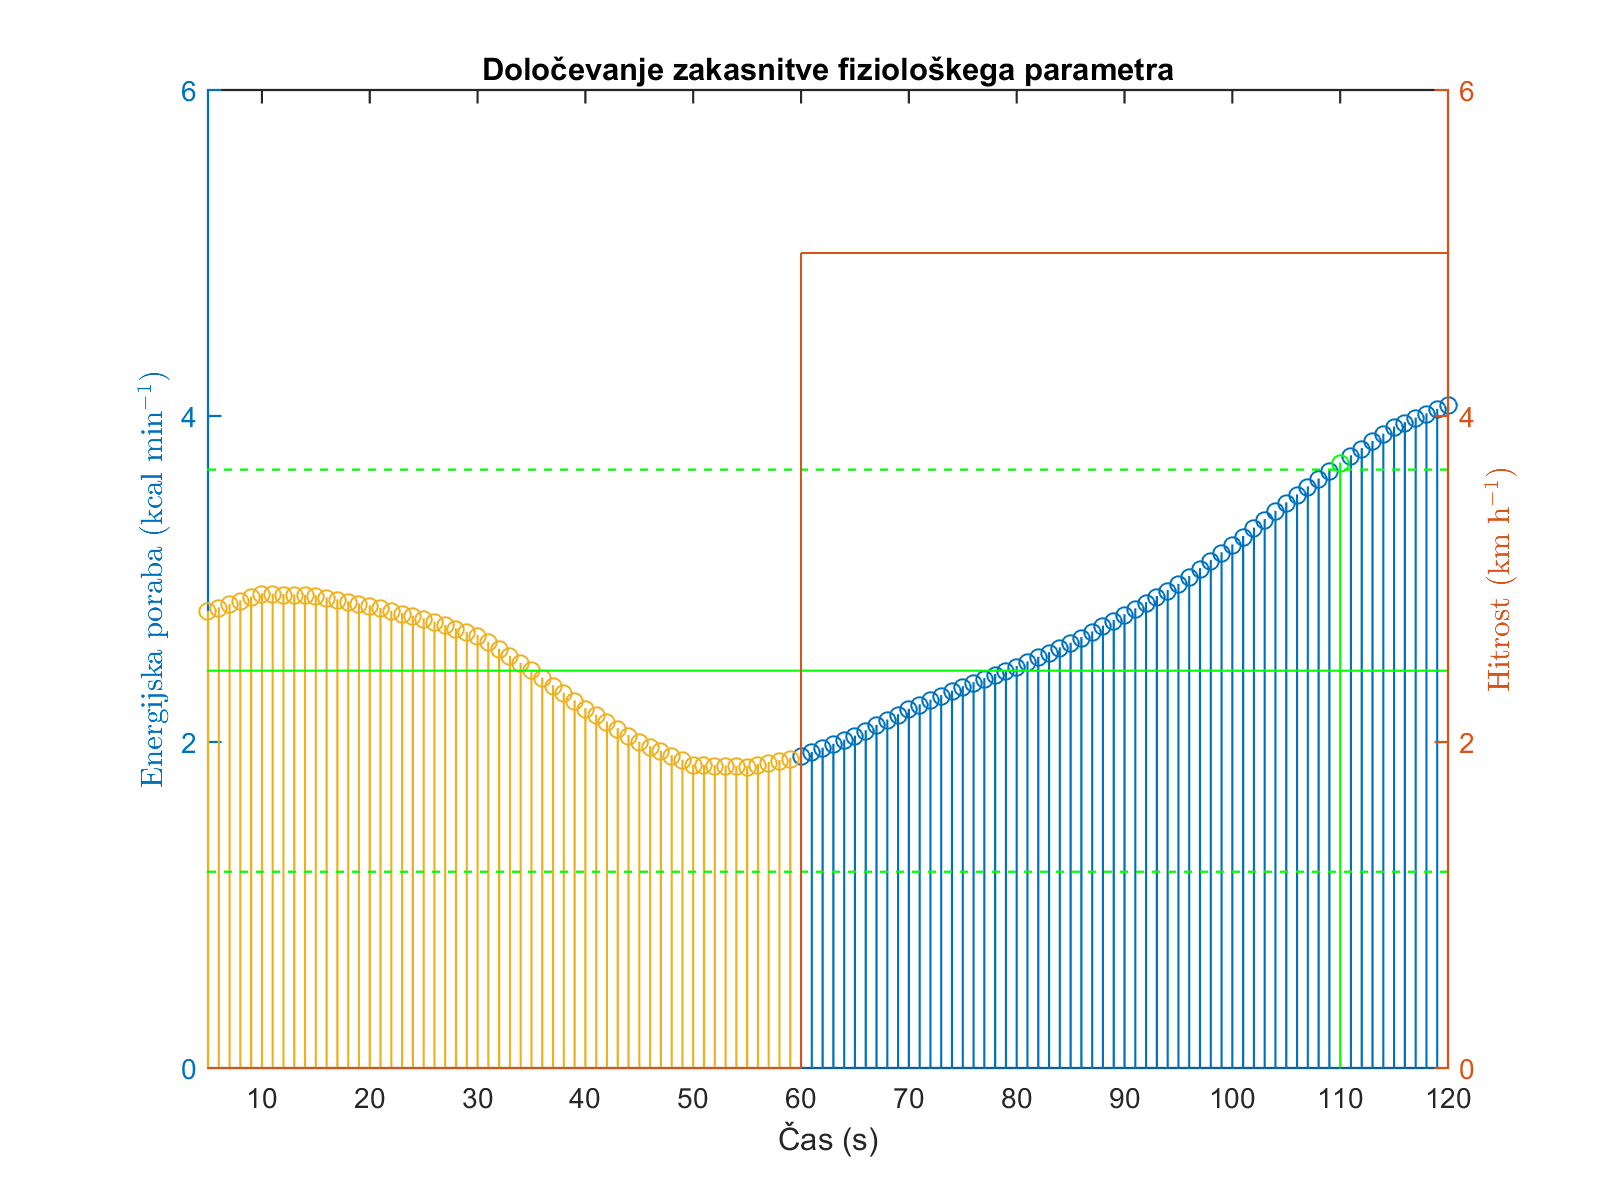
\includegraphics[width=\columnwidth]{./Slike/lag-estimation-6-eem.png}
\caption{Zakasnitev za subjekt 6.}
\label{fig:lag-estimation-train-eem}
\end{subfigure}
\caption{}
\label{fig:lag-estimation-stage1}
\end{figure}



\subsection{Optimizacija Gaussovega filtra}
Pri optimizaciji Gaussovega filtra smo določili optimalni standardni odklon $\sigma$ z uporabo dveh metrik, in sicer: koren srednje kvadratične napake (RMSE) in razmerje med signalom in šumom (SNR). Pri RMSE metriki smo določili napako med učnimi vzorci in njihovo predikcijo. Pri SNR metriki smo za signal uporabili referenčne učne vzorce. Za šum smo uporabili rezidualni ali preostali šum. Tega smo dobili z odštevanjem filtriranih vzorcev od referenčnih. SNR metrika tako določa uspešnost izločevanja šuma, RMSE metrika pa pravilnost določevanja kateri podatki spadajo v signal in kateri v šum.


Teste smo izvajali na vseh eksperimentih 1. sklopa, pri čemer smo uporabili $\nu$-RBF jedro s \SI{50}{\%} podpornih vektorjev. Za filtriranje pri mrežnem iskanju smo izbrali najmanjši filter s $\sigma = 1$. Testirali smo naslednje standardne odklone Gaussovega filtra: $1, 3, 5, 11, 21, 31$ in $51$. 

Rezultati povrprečnih vrednosti uporabljenih metrik so vidni v tabeli \ref{tab:gauss}. Za pravilno razlago rezultatov, moramo upoštevati tudi grafe metrik posameznih eksperimentov, ki so prikazani na slikah \ref{fig:sigma1-5}, \ref{fig:sigma-rmse5-21} in \ref{fig:sigma21-51}. 



\begin{table}[htb]
	\centering
    \begin{tabular}{S[table-format=2.0] S[table-format=2.3] S[table-format=2.3]}
    \toprule
    \thead{$\mathbf{\sigma}$} & \thead{RMSE} & \thead{SNR [dB]}  \\
    \midrule%nSV
    1 & \boldentry{2.3}{8.614} & 24.278 \\
    3 & 11.236 & 25.470 \\
    \boldentry{2.0}{5} & 11.596 & 25.746 \\
    11 & 11.783 & 25.746 \\
    21 & 11.842 & 25.975 \\
    31 & 11.871 & 26.194 \\
    51 & 11.907 & \boldentry{2.3}{26.306} \\
    \bottomrule
    \end{tabular}
    \caption[Povprečne vrednosti RMSE in SNR metrik pri optimizaciji parametra $\sigma$ Gaussovega filtra]{Povprečne vrednosti RMSE in SNR metrik pri optimizaciji parametra $\sigma$ Gaussovega filtra. Najmanjši standardni odklon ima najmanjšo napako, vendar je tudi filtriranje majhno. Pri $\sigma=3$ in $\sigma=5$ so še opazne razlike pri filriranju. Za višje vrednosti ni več opazne razlike, vendar pa se napaka povečuje. $\sigma=5$ je tako optimalna vrednosti parametra.}
    \label{tab:gauss}
\end{table}

Najmanjšo napako dobimo, če uporabimo $\sigma=1$, vendar pa imamo pri tem najmanjše filtriranje, zato so rezultati še vedno lahko zelo šumni. Z višanjem parametra filtra, se napaka po metriki RMSE povečuje, vendar ima večji vpliv razmerje SNR, saj je predstavljeno v logaritemski skali. 

\begin{figure}[htb]
\centering
\begin{subfigure}[t]{0.45\columnwidth}
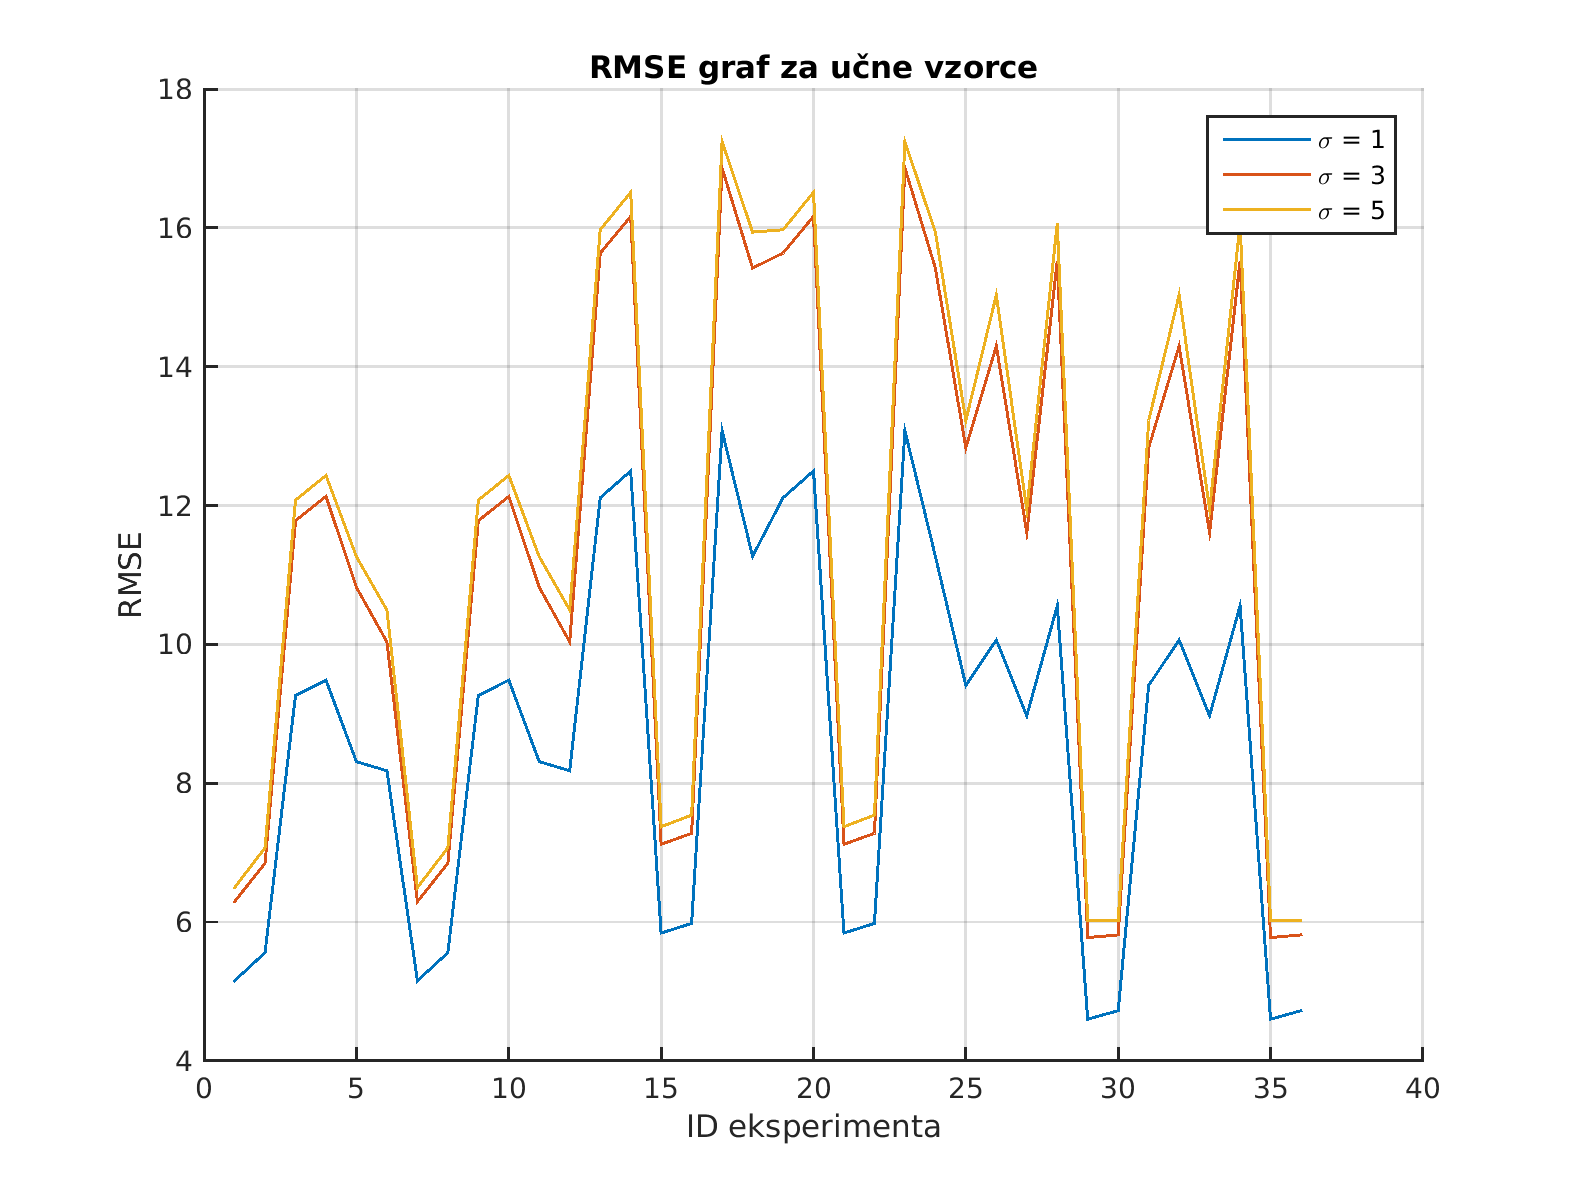
\includegraphics[width=\columnwidth]{./Slike/sigma-rmse1-5.png}
\caption{Graf RMSE  učnih vzorcev }
\label{fig:sigma-rmse1-5}
\end{subfigure}
~
\begin{subfigure}[t]{0.45\columnwidth}
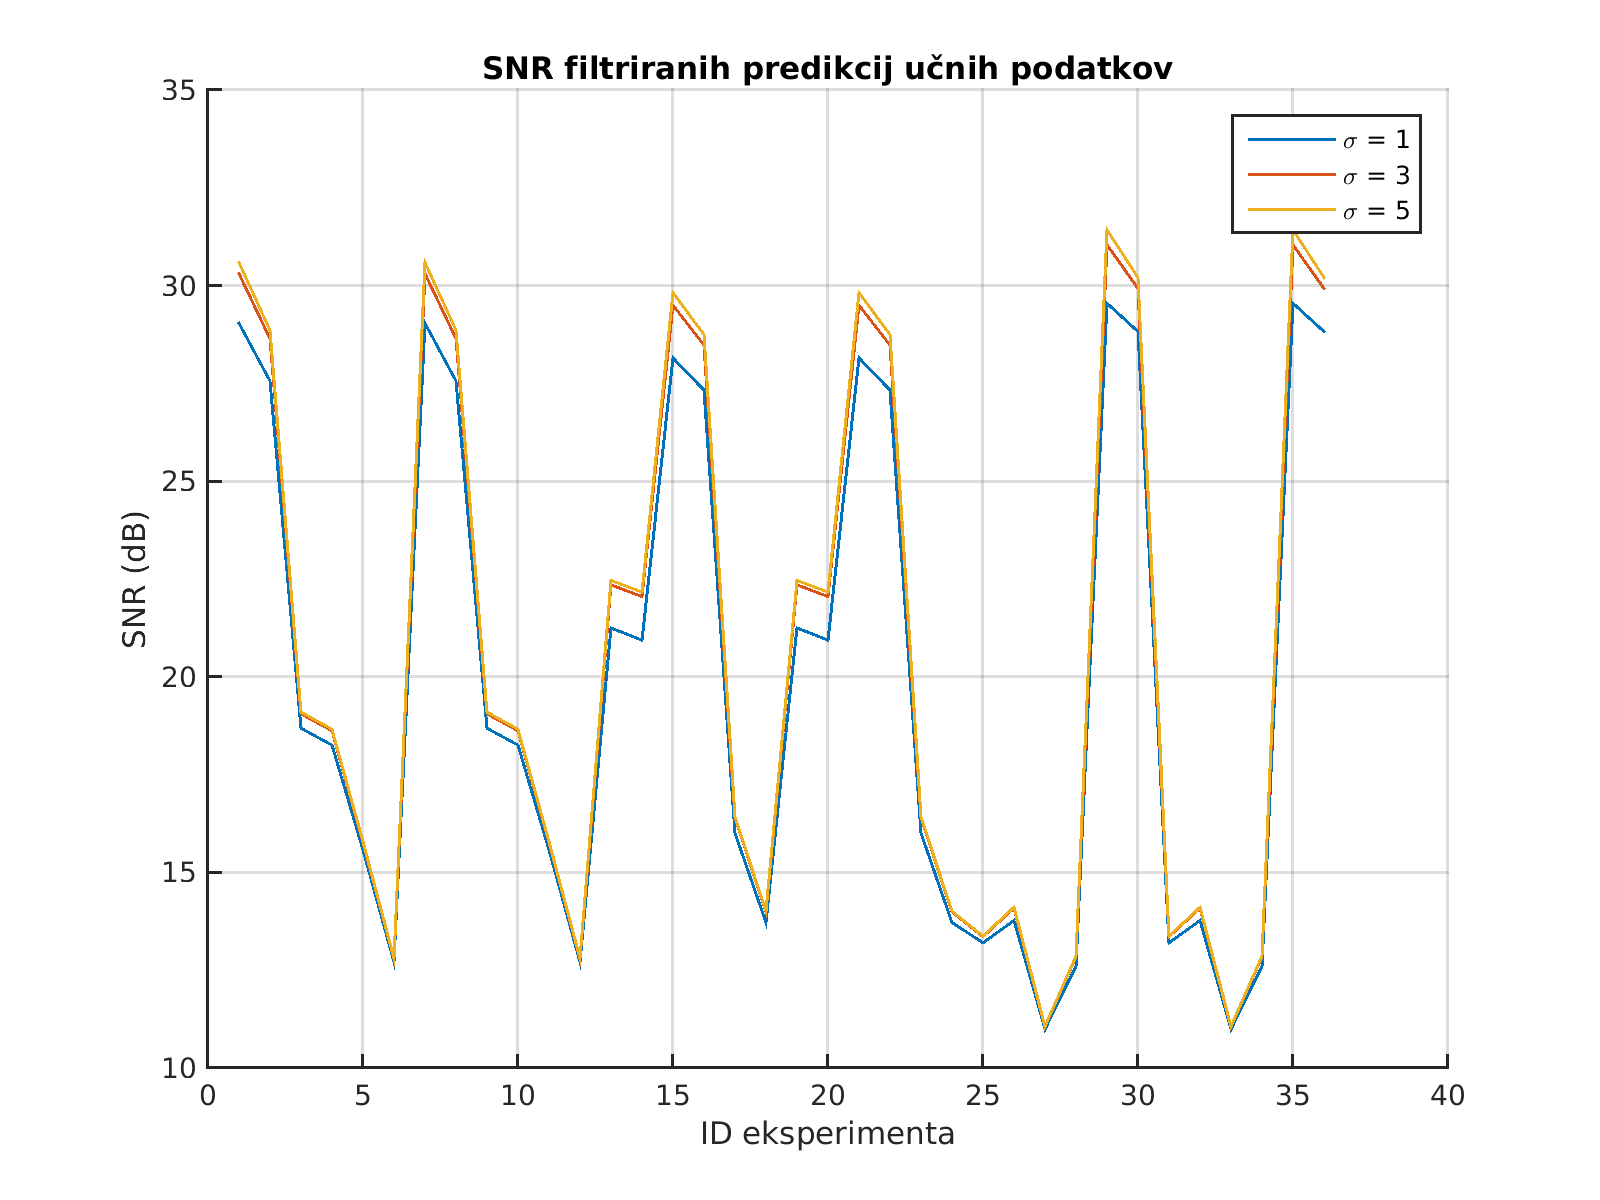
\includegraphics[width=\columnwidth]{./Slike/sigma-snr1-5.png}
\caption{Graf SNR  učnih vzorcev}
\label{fig:sigma-snr1-5}
\end{subfigure}
\caption{Grafa RMSE in SNR učnih vzorcev za \mbox{$\sigma \in [1,5]$}}
\label{fig:sigma1-5}
\end{figure}

Čeprav pri uporabi $\sigma=51$ dobimo največje filtriranje šuma, lahko na slikah grafov opazimo, da se obe metriki bistveno ne razlikujeta za vrednosti parametra na intervalu $[5,51]$. Kljub dobremu filtriranju želimo zagotoviti čim manjšo napako med referenčnim signalom in predikcijo, zato je logična izbira čim manjši standardni odklon. Ker so na sliki \ref{fig:sigma1-5} med $\sigma=3$ in $\sigma=5$ še opazne razlike, lahko zaključimo, da je $\sigma=5$ optimalna izbira parametra za naš problem. 


\begin{figure}[htb]
\centering
\begin{subfigure}[t]{0.45\columnwidth}
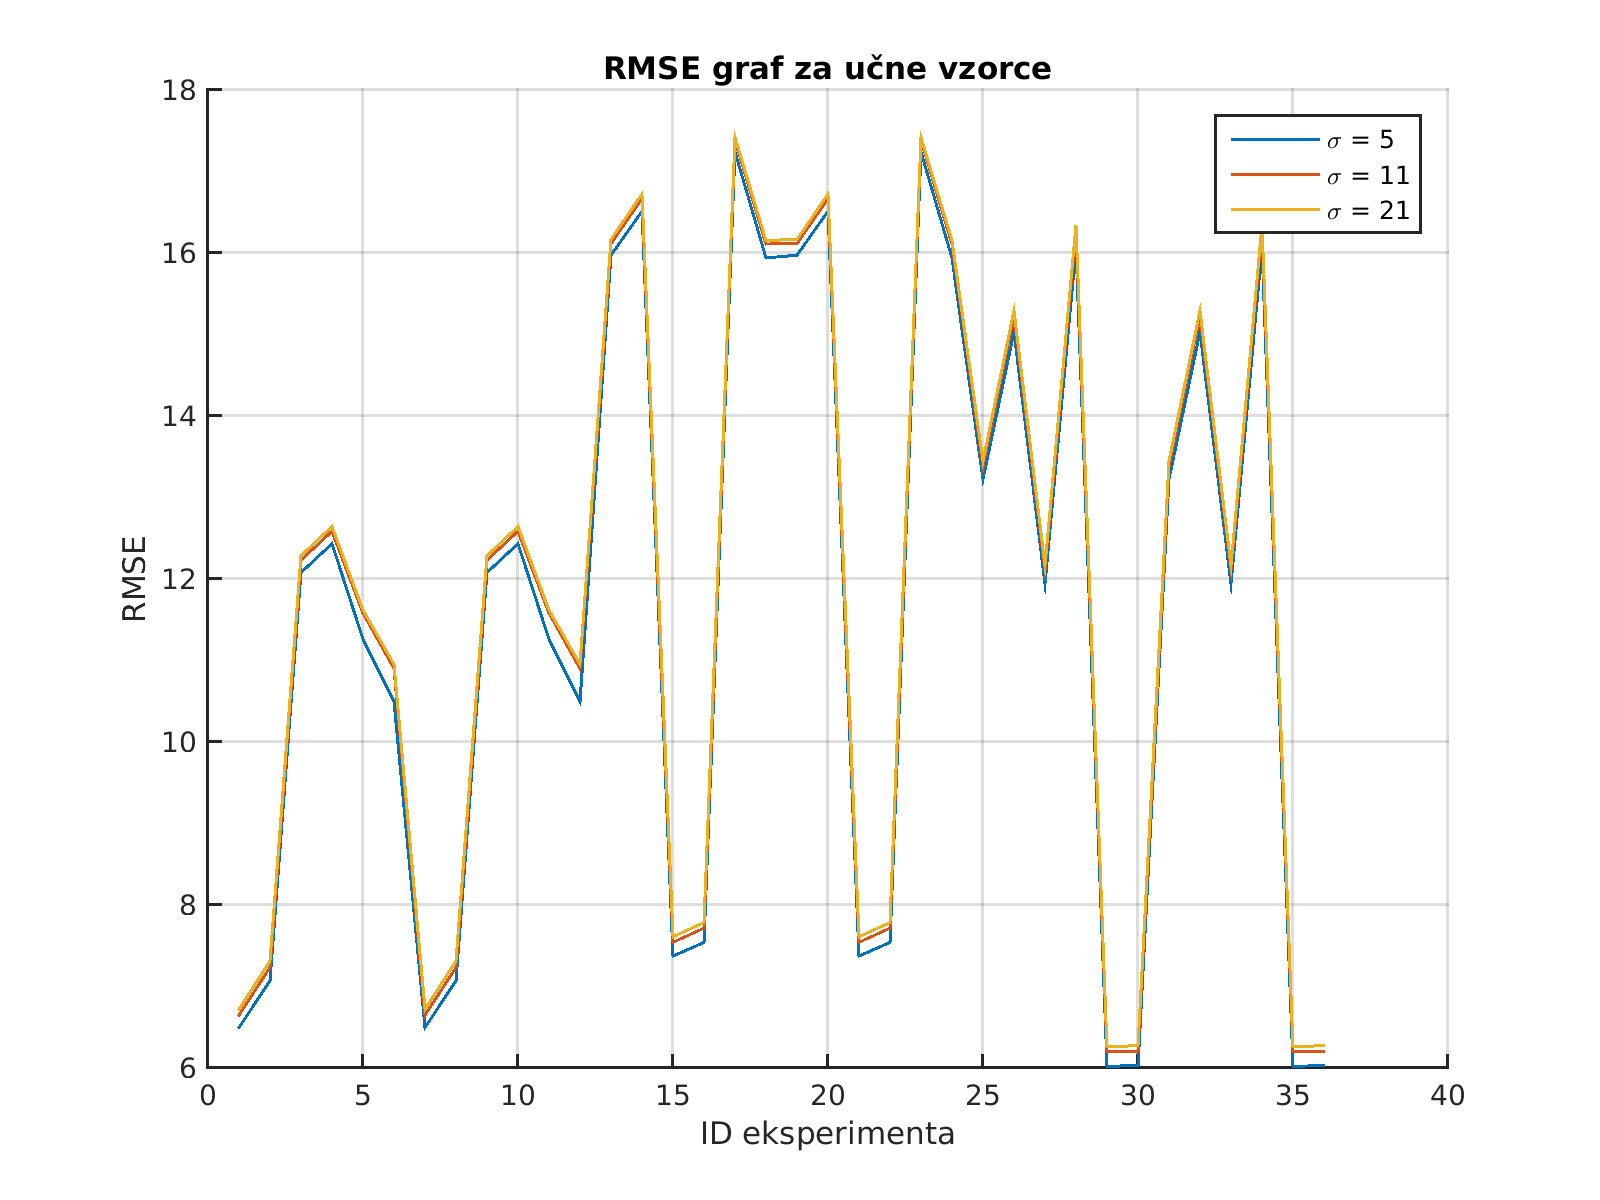
\includegraphics[width=\columnwidth]{./Slike/sigma-rmse5-21.png}
\caption{Graf RMSE  učnih vzorcev}
\label{fig:sigma-rmse5-21}
\end{subfigure}
~
\begin{subfigure}[t]{0.45\columnwidth}
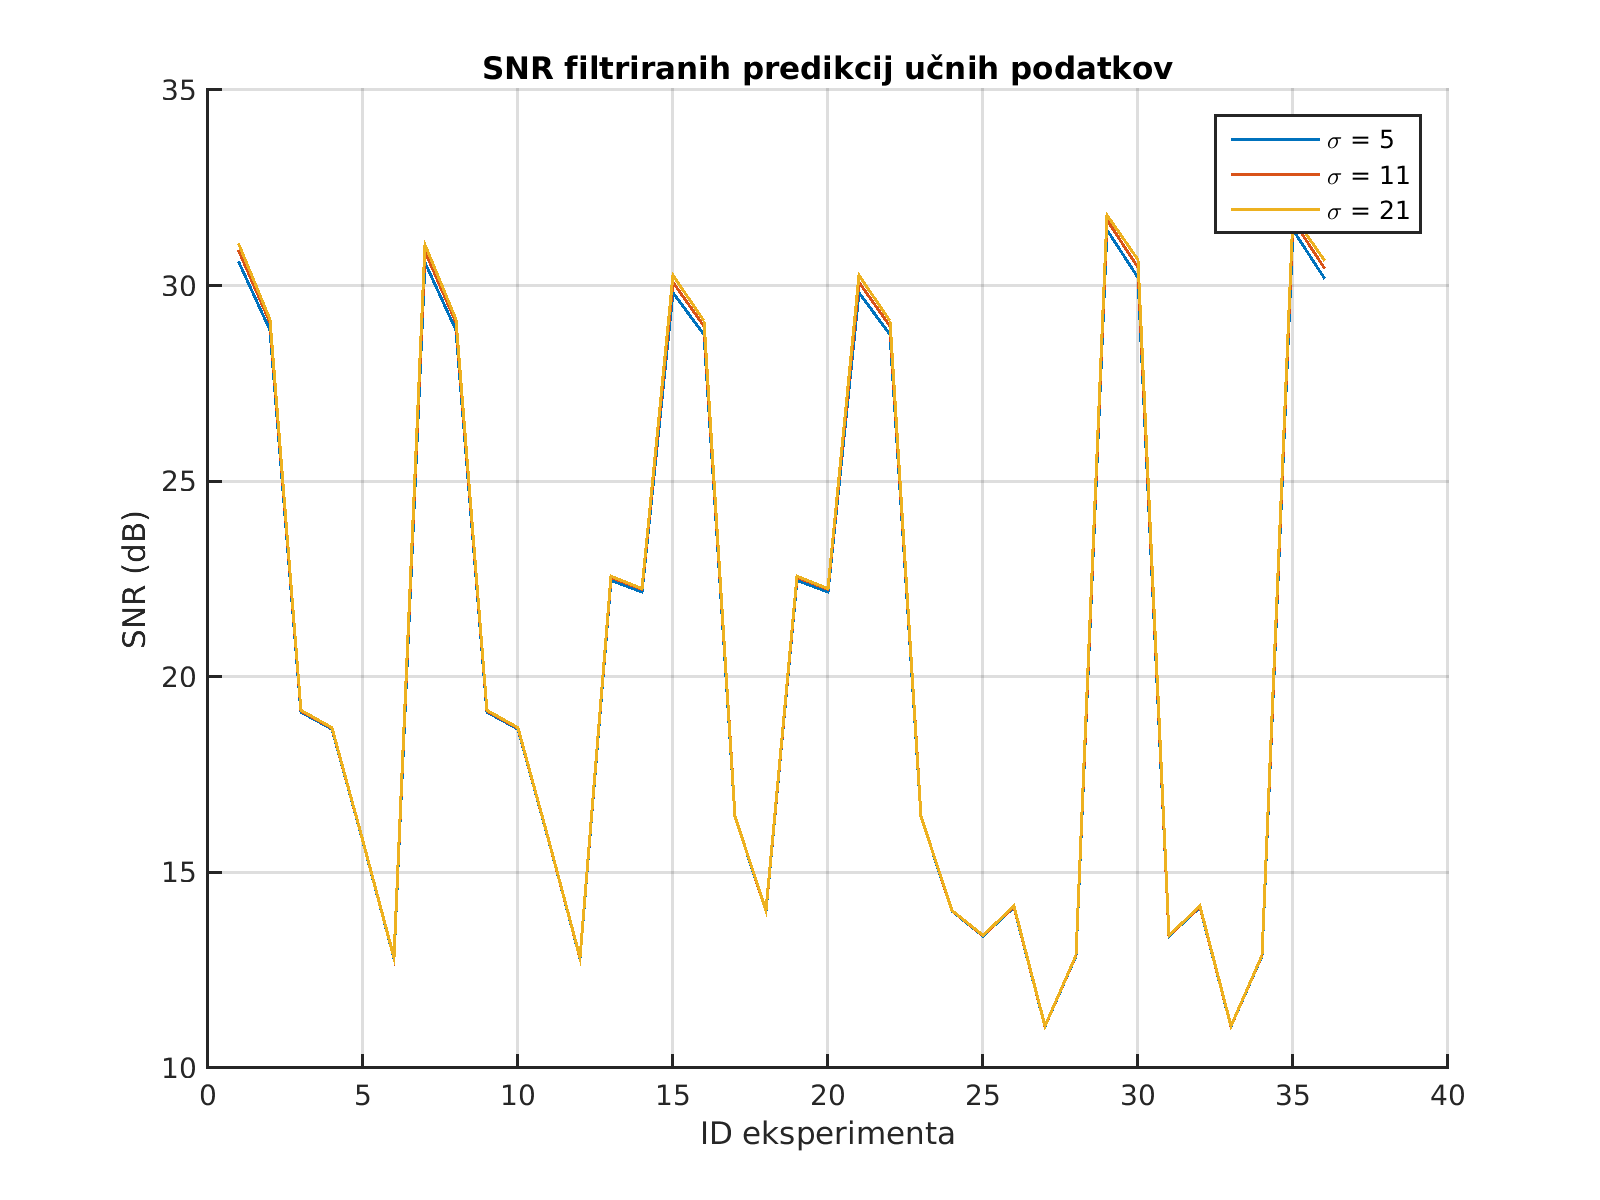
\includegraphics[width=\columnwidth]{./Slike/sigma-snr5-21.png}
\caption{Graf SNR  učnih vzorcev}
\label{fig:sigma-snr5-21}
\end{subfigure}
\caption{Grafa RMSE in SNR učnih vzorcev za \mbox{$\sigma \in [5,21]$}}
\label{fig:sigma5-21}
\end{figure}



\begin{figure}[htb]
\centering
\begin{subfigure}[t]{0.45\columnwidth}
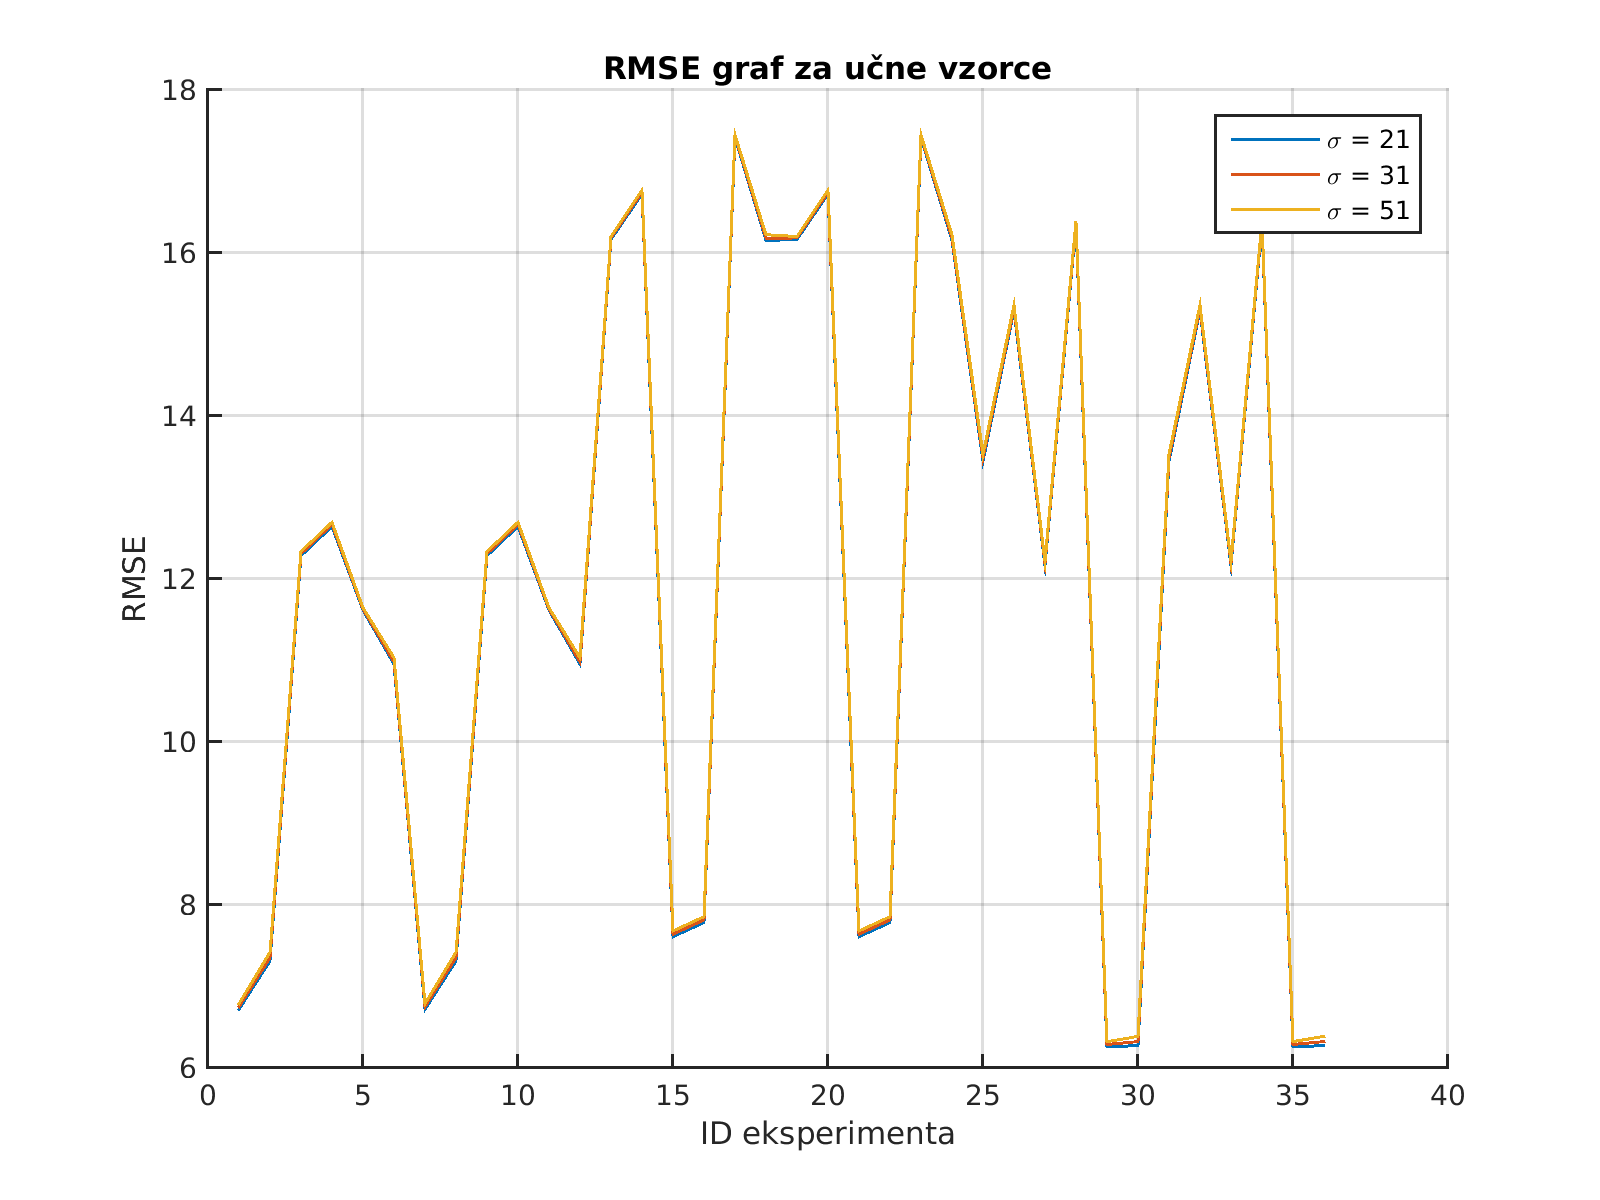
\includegraphics[width=\columnwidth]{./Slike/sigma-rmse21-51.png}
\caption{Graf RMSE učnih vzorcev}
\label{fig:sigma-rmse21-51}
\end{subfigure}
~
\begin{subfigure}[t]{0.45\columnwidth}
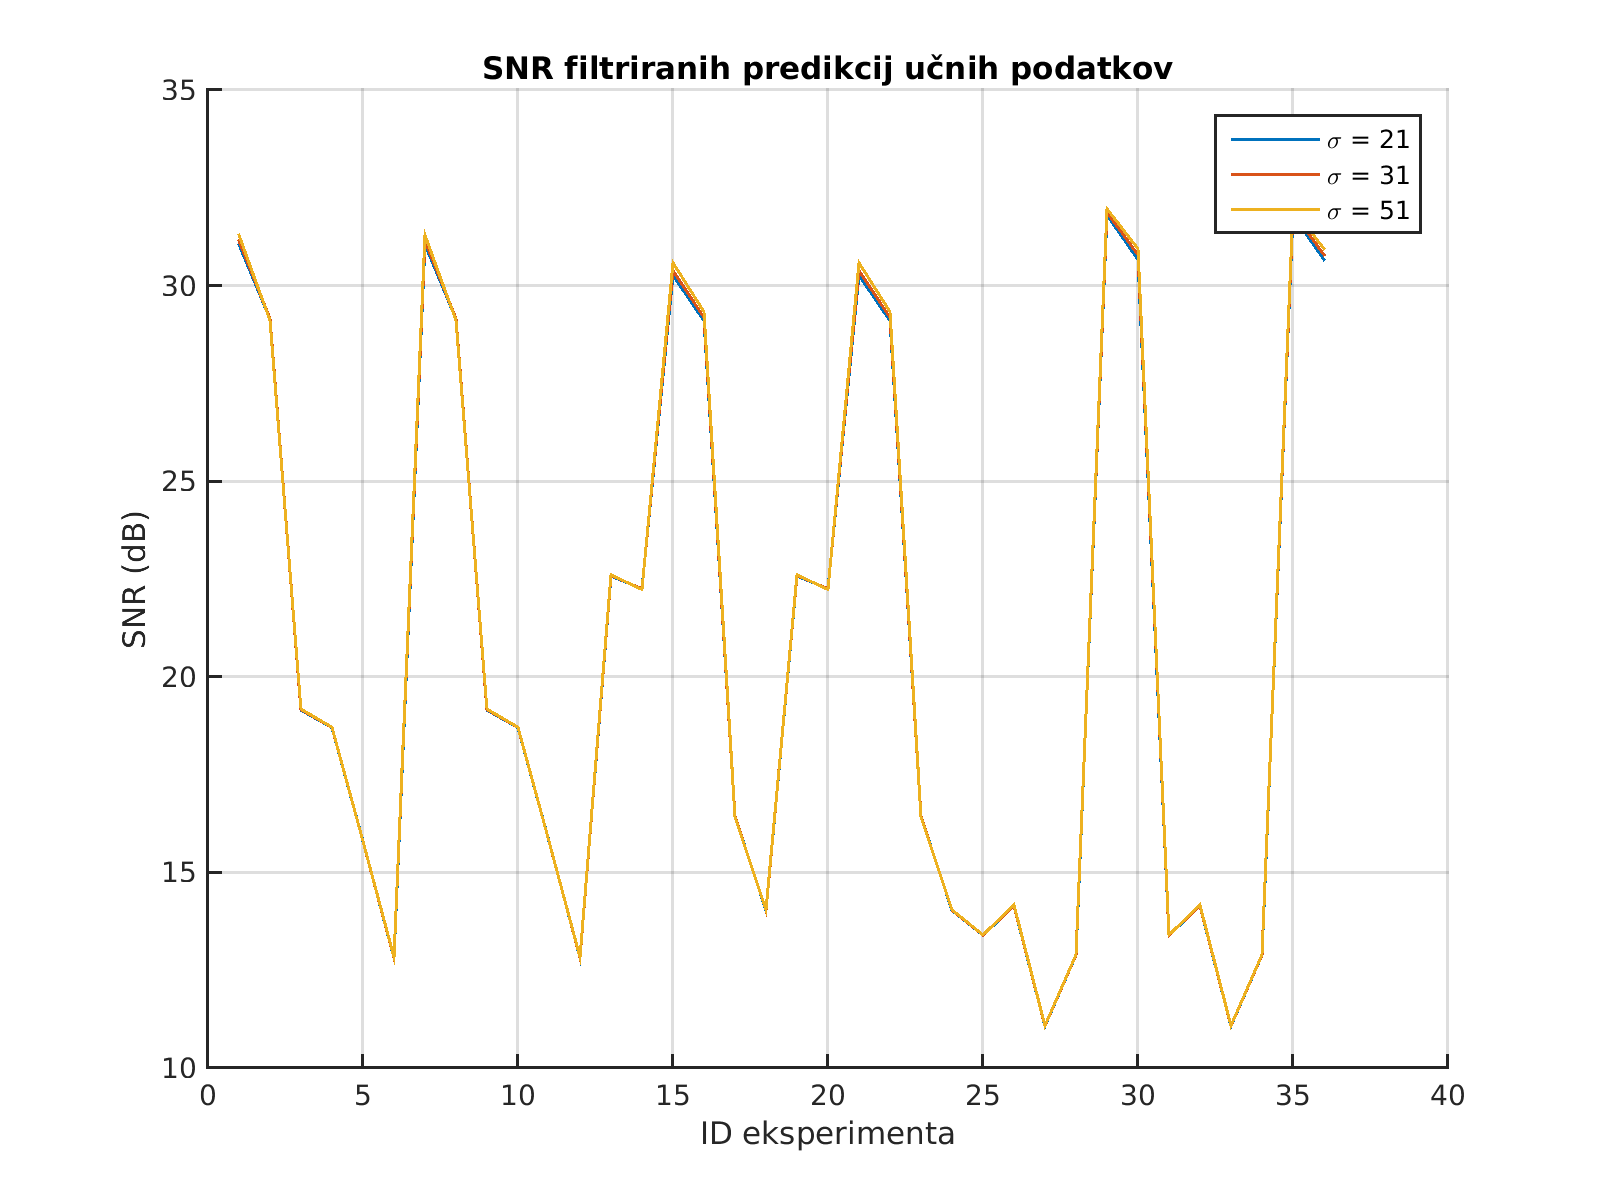
\includegraphics[width=\columnwidth]{./Slike/sigma-snr21-51.png}
\caption{Graf SNR  učnih vzorcev}
\label{fig:sigma-snr21-51}
\end{subfigure}
\caption{Grafa RMSE in SNR učnih vzorcev za \mbox{$\sigma \in [21,51]$}}
\label{fig:sigma21-51}
\end{figure}


\subsubsection{Regresija \texorpdfstring{$\nu$}{nu}-RBF}



\subsection{Laboratorijski eksperimenti}
a

\subsection{Terenski eksperimenti}
a
